\documentclass[a4paper]{article}

\usepackage{inputenc}
\usepackage[british,UKenglish]{babel}
\usepackage{amsmath}
%\usepackage{titlesec}
\usepackage{color}
\usepackage{graphicx}
\usepackage{fancyref}
\usepackage{hyperref}
\usepackage{float}
\usepackage{scrextend}
\usepackage{setspace}
\usepackage{xargs}
\usepackage{multicol}
\usepackage{nameref}

\usepackage{sectsty}
\usepackage{multicol}
\usepackage{multirow}
\usepackage[procnames]{listings}
\usepackage{appendix}
\usepackage{listings}
\usepackage{caption}
\usepackage{multirow}

\usepackage{cite}
\bibliographystyle{IEEEtran}

\newcommand\tab[1][1cm]{\hspace*{#1}}
\hypersetup{colorlinks=true, linkcolor=black}
\interfootnotelinepenalty=10000

\newcommand{\cleancode}[1]{\begin{addmargin}[3em]{3em}\texttt{\textcolor{cleanOrange}{#1}}\end{addmargin}}
\newcommand{\cleanstyle}[1]{\text{\textcolor{cleanOrange}{\texttt{#1}}}}


\usepackage[colorinlistoftodos,prependcaption,textsize=footnotesize]{todonotes}
\newcommandx{\commred}[2][1=]{\textcolor{Red}
{\todo[linecolor=red,backgroundcolor=red!25,bordercolor=red,#1]{#2}}}
\newcommandx{\commblue}[2][1=]{\textcolor{Blue}
{\todo[linecolor=blue,backgroundcolor=blue!25,bordercolor=blue,#1]{#2}}}
\newcommandx{\commgreen}[2][1=]{\textcolor{OliveGreen}{\todo[linecolor=OliveGreen,backgroundcolor=OliveGreen!25,bordercolor=OliveGreen,#1]{#2}}}
\newcommandx{\commpurp}[2][1=]{\textcolor{Plum}{\todo[linecolor=Plum,backgroundcolor=Plum!25,bordercolor=Plum,#1]{#2}}}

\def\code#1{{\tt #1}}

\def\note#1{\noindent{\bf [Note: #1]}}

\makeatletter
%% The "\@seccntformat" command is an auxiliary command
%% (see pp. 26f. of 'The LaTeX Companion,' 2nd. ed.)
\def\@seccntformat#1{\@ifundefined{#1@cntformat}%
   {\csname the#1\endcsname\quad}  % default
   {\csname #1@cntformat\endcsname}% enable individual control
}
\let\oldappendix\appendix %% save current definition of \appendix
\renewcommand\appendix{%
    \oldappendix
    \newcommand{\section@cntformat}{\appendixname~\thesection\quad}
}
\makeatother



\lstset{frame=, basicstyle={\footnotesize\ttfamily}}

\graphicspath{ {images/} }
\usepackage{ctex}
\usepackage{bm}
%-----------------------------------------BEGIN DOC----------------------------------------

\begin{document}
\renewcommand{\contentsname}{目\ 录}
\renewcommand{\appendixname}{附录}
\renewcommand{\appendixpagename}{附录}
\renewcommand{\refname}{参考文献} 
\renewcommand{\figurename}{图}
\renewcommand{\tablename}{表}
\renewcommand{\today}{\number\year 年 \number\month 月 \number\day 日}
\begin{titlepage}
\title{{\Huge \textbf{网络数据挖掘}{\large\linebreak\\}}{\Large \textbf{垃圾短信识别}\linebreak\linebreak}}
%please write your name, Student #, and Class # in Authors, student ID, and class # respectively


\author{\\
\\ \\ \\ \\ \\ \\
\textbf{XXX 2018180132290**}  \\
\\ \\ \\ \\ \\ \\ \\  \\ \\  \\ \\ \\ \\}

\date{\today}

\maketitle
\thispagestyle{empty}
\end{titlepage}


\newpage

\thispagestyle{empty}
\begin{center}
\tableofcontents\label{c}
\end{center}
\thispagestyle{empty}
\setcounter{page}{0}
\newpage

%------------------------------------------TEXT--------------------------------------------

%----------------------------------------OVERVIEW-----------------------------------------
\section{介绍}

\subsection{背景}
假定我们现有一封短信,其内容如下:
\textit{一次价值xxx元王牌项目;可充值xxx元店内项目卡一张;可以参与V动好生活百分百抽奖机会一次!预约电话:xxxxxxxxxxx}充斥着各种诱人的促销信息,很有可能是一封垃圾短信。现在各个网站与App都鼓励人们用手机号进行注册,手机号已经不再是一个非常私人的信息。据《2013年垃圾短信报告》称,去年中国手机用户收到的垃圾短信总量超过2000亿条,给全国手机用户造成超过上亿元的经济损失。而伪基站自去年7月出现后逐渐增多,已经成为垃圾短信尤其是诈骗短信孳生的温床。

迄今为止 ,垃圾短信在国际上并没有一个标准的定义。其基本特征是“不请自来”,而且大部分垃圾短信都带有商业或者其他宣传目的\cite{王斌2005基于内容的垃圾邮件过滤技术综述}。要解决垃圾短信问题,必须综合法律、技术等手段。反垃圾短信技术上可以分成两类:“根源阻断”和“存在发现”。“根源阻断”是指通过防止垃圾短信的产生来减少垃圾短信,该方法目前还没得走向实用。目前,主流的反垃圾短信技术是“存在发现”,即对存在的短信进行识别分类。垃圾短信识别可以通过对短信文本分类来实现。

一直以来,垃圾邮件分类(Spam)都是文本分类问题的一个经典而又重要的任务,本项目的垃圾短信分类,从本质上说和垃圾邮件分类属于同一任务,报告中垃圾短信和垃圾邮件是通用的。

\subsection{与其他任务的异同}
\subsubsection{图像分类}
图像分类是一项发展历史悠久的技术,它的基本任务可以概括为,建立一个从图像域$X$到标签域$Y$的映射,从这个抽象的角度看,图像分类问题和文本分类问题异曲同工。通常而言,解决分类问题可以分为两步,首先是对数据域$X$进行特征提取,然后利用提取到的特征进行分类。在传统方法中,这两步是分离进行的,而在深度学习方法则是统一的,通常可以将神经网络的最后一层看作分类器,其他隐层则起到特征提取的作用。

尽管抽象层次上,图像分类问题和文本分类问题是统一的,但在细节上存在诸多差异,主要集中于特征提取部分。首先,图像和文本的组成粒度不同。图像是由大量低层次的像素构成,而文本则由高层次的词语组成。另外,图像中,像素的组合呈现出空间性;而文本中,词语被组合成序列的形式,且在本质上,词语的组合是树形的,组成粒度以及组合方式的不同导致了图像分类和文本分类特征提取的巨大差异。传统方法中,图像分类常常提取HOG、SURF、LBP等特征,而文本则提取如TF-IDF,或将文本组成词袋的形式,或提取n-gram特征。在深度学习方法中,卷积神经网络的应用和发展为图像分类带来了爆炸性的进展,通过在图像上运行卷积神经网络,模型可以层次性地提取到从低层的纹理到高层的目标等等诸多特征。而在文本分类方面,词向量技术的引入使得文本分类可以像图像分类一样,在更低的层次进行特征提取,并且考虑词语组合方式的特殊性,循环神经网络被引入用于挖掘文本的特征。

\subsubsection{推荐系统}

推荐系统的起源可追溯到近20年前,但直到至今推荐系统依然没有一个非常精确的定义,广义上的推荐系统可以理解为是主动向用户推荐物品(Item)的系统,所推荐的物品可以是是音乐、书籍、餐厅、新闻条目等等,这依赖于具体的应用领域。

从某些角度,推荐问题可以形式化地定义为一个特征高度稀疏的分类问题\cite{herlocker1999algorithmic},并利用协同过滤技术求解。而在用户和物品均有大量描述属性的情形下,用户和物品的特征可以由其高度稀疏的编号的独热编码以及其描述属性所构成,并利用混合推荐技术求解,同样地,适用于文本分类的分类器可以在这一场景下使用。除此之外,当用户或物品存在文本形式的特征时,文本分类所用到的一系列进行文本处理的技术会被推荐系统所使用。

近年来,随着深度学习技术在推荐系统中得到广泛地应用,推荐系统中的协同过滤方法愈加类似于自然语言处理领域的词向量技术,如文献\cite{he2017neural}将物品和用户编号映射到低维的Embedding空间,并在其上构建多层感知机,文献\cite{barkan2016item2vec}中,Word2vec算法被用于用户交互过的物品序列中,用于学习物品的向量化表示。

除了这些相似点,推荐系统与文本分类还存在着更多的差异,如推荐系统所面临的冷启动问题,丰富且跨媒体的特征,如电影推荐中的电影剧照,电影描述,用户档案等,海量数据以及极高维极稀疏特征(上亿维)等等,这些都是文本分类问题所不具备的。




\subsection{模型选择}
垃圾短信分类可以看作一个文本分类问题,即正常短信与垃圾短信。我们考虑使用常用文本分类技术来解决该任务。因此, 各种文本分类方法都可以用于垃圾短信的分类,而基本上大部分机器学习方法都在文本分类领域有所应用,如:朴素贝叶斯分类算法、KNN、SVM、最大熵和神经网络等等。

垃圾短信分类任务的特点是语料多且粗糙杂乱、非垃圾短信要远多于垃圾短信,即数据不平衡。根据以上特点,可以选择稳定性较高以及适用于大量数据不易欠拟合的模型。本项目经过尝试了6种算法,包括经典的机器学习算法:易于实现的逻辑回归(Logistic Regression,LR),稳定性很高的朴素贝叶斯\cite{sahami1998bayesian}(Naive Bayes,NB),支持向量机\cite{tong2001support}(Support Vector Machine,SVM),适用于大量数据的随机森林\cite{breiman2001random}(Random Forest,RF); 和深度学习算法:特征提取能力强大的卷积神经网络\cite{kim2014convolutional}(Convolutional Neural Network,CNN),能够学习长期依赖的循环神经网络\cite{sundermeyer2012lstm}(Recurrent Neural Network,RNN)。

\subsection{章节安排}
第一章为引言部分,介绍了当前垃圾短信泛滥的形势,提出研究垃圾短信分类任务的重要意义,该任务实际上是文本分类任务,介绍了它与其他任务的相同与不同点,选择模型的原因以及主要工作。

第二章介绍了文本分类任务的相关工作。首先介绍了经典的机器学习方法,在分类器设计方面与特征提取方面的研究现状;然后介绍了深度学习方法应用于文本分类工作现状。为本文之后使用的模型打下基础。

第三章介绍了本项目的文本预处理部分,使用正则化,分词,词向量化等方式,将原始语料处理成便于应用机器学习算法的相对规则化的数据。

第四章介绍了特征提取方式,使用了TF-IDF特征,哈希特征,用于经典的机器学习算法。

第五章模型部分,介绍了本项目使用的模型理论依据,共有六个模型,并对比了他们各自的优缺点。包括:经典的机器学习算法逻辑回归、朴素贝叶斯、支持向量机、随机森林,与深度学习算法CNN和LSTM。

第六章实验和Demo部分,介绍了实验的数据集划分评价指标,各个模型参数设置,实验的结果和分析比较。并介绍了Demo的前后端以及使用说明。


\section{相关调研} \label{relatedwork}%------------------------------
目前对于垃圾邮件识别的研究主要集中在利用邮件的内容来区分垃圾邮件,即利用文本分类技术将垃圾邮件识别问题转化为一个有监督的学习问题\cite{r1}。国外的文本分类研究开始于20世纪50年代末,早期的文本分类需要人为定义分类规则,效果不尽如人意。随着机器学习的发展,人们将机器学习的技术应用到文本分类中,首先对已经过人工标注的文本进行特征提取,然后利用算法对文本进行自动分类。这一技术为文本分类领域带来了突破性的进展,也促使了文本分类领域新的研究成果的不断涌现。研究者们主要聚焦于文本分类领域的两个重要方面,分类器的设计和文本特征提取。

在分类器设计方面,研究者们比较了不同的分类器在垃圾邮件识别问题上性能的差异,
W.A. Awad等人\cite{r5}等人在SpamAssassin数据集上比较了Naive Bayes、SVM、KNN、Rough sets等方法的性能差异,得出Naive bayes和Rough sets方法比其他方法在分类正确率上表现更好的结论;Aman Kumar Sharma\cite{sharma2011comparative}在UCI数据集上比较了ID3、CART、ADTree、J48等方法在垃圾邮件分类正确率上的表现,J48方法取得了最好结果;Bhagyashri U. Gaikwad\cite{Bhagyashri_ijacect}等人将集成学习中的Random forests应用于垃圾邮件分类,在csmining的spam-email-datasets上进行实验,在TPR及FPR上得分较高;Xavier Carreras等人\cite{carreras2001boosting}将Adaboost方法应用于垃圾邮件分类,在PU1数据集上进行实验,结果表明该方法比Decision Trees及 Naive Bayes方法可以获得更优的F1-score;Mathew等人则在SMS短信领域进行了研究\cite{mathew2011intelligent},并比较了包括贝叶斯网络、多层感知机、受限玻尔兹曼在内的超过30种分类器的性能,得到了多项式朴素贝叶斯分类器效果最好的结论。

在特征提取方面,陶峰等人\cite{tf_tfidf}注意到TFIDF算法没有考虑到算法并没有考虑到特征词在类间的分布情况的缺陷,对TFIDF算法进行了改进;李猛等人\cite{lm_ig}改进了信息增益算法未分析特征项在类内和类间分散程度的缺陷;王禾清\cite{whq_mi}则针对互信息特征选择方法缺少词频信息的缺陷,对传统的互信息方法进行了改进,并针对二分类问题,引入了特征贡献比的概念。除此之外,研究者们还比较了不同的特征提取方法在垃圾邮件识别问题上的性能差异。赵晓丹等人\cite{zxd}等人比较了在朴素贝叶斯分类器和SVM分类器下,文档频率、信息增益、互信息、卡方统计量和优势率等特征提取方法的效果,实验结果显示优势率、卡方统计量和信息增益最优。

近年来,深度学习技术也开始应用于文本分类领域,并取得了超越传统分类方法的效果。Mikolov等人\cite{mikolov2013distributed}提出了word2vec模型,能够在大规模的未标注语料库上训练词向量,解决了词汇鸿沟问题的同时,还使得大规模语料库的信息能够传递至小规模数据集上。Petters等人\cite{peters2018deep}则提出了ELMO,利用了双向的长短期记忆网络来训练语言模型,并利用在大规模的未标注语料库上训练得到的预训练语言模型作为下游任务的特征提取模型,大大提升了文本分类以及其他自然语言处理领域下游任务的性能。在文本分类的模型架构设计方面,Kim\cite{kim2014convolutional}将卷积神经网络应用于文本分类,Zhang等人\cite{zhang2015character}等人提出了一个字级别的卷积神经网络,能够利用字级别的信息并解决OOV问题,在实验上超过了传统方法以及其他基于深度学习的方法。

%------------------------------
\section{文本处理}

本任务使用的原始语料是是非格式化数据,比较杂乱,粗糙,同时中文文本没有间隔符,难以直接进行研究使用。需要进行文本预处理,使用一些正则化方法来将原始语言转换为规则的、易于处理的文本,然后进行分词,同时深度学习需要将文本变为词向量\cite{周钦强2005文本自动分类系统文本预处理方法的研究}。同时中文编码不是utf-8,需要再打开文件的时候以utf-8格式打开。
\subsection{正则化}
原始语料比较粗糙,包含繁体字符、数字、中文标点,英文单词大小写都有。需要进行正则化处理,调用python中的re模块。
\begin{enumerate}
	\item 繁简体正则化:使用 繁简体字符对照表,将繁体字符转化为简体字。
	\item 标点符号正则化:利用建立的标点对照表将中文字符转化为英文字符,同时去掉连续的空格,与连续的点。
	\item 英文字符正则化:将大写字母转化为小写。
\end{enumerate}


\subsection{分词}
中文文本分类时,由于词语间没有分隔,需要分词才能提取文本特征词语。现有的中文分词方法大致可分为基于词典、基于统计和基于自然语言理解三类方法。

目前已经有可用性比较好的分词解决方案,大多使用机器学习算法和词典相结合,一方面能够提高分词准确率,另一方面能够改善领域适应性。本项目的中文分词方案采用结巴分词Python版\footnote{https://github.com/fxsjy/jieba},结巴分词提供三种分词模式:
\begin{enumerate}
	\item 精确模式,试图将句子最精确地切开,适合文本分析;
	\item 全模式,把句子中所有的可以成词的词语都扫描出来, 速度非常快,但是不能解决歧义;
	\item 搜索引擎模式,在精确模式的基础上,对长词再次切分,提高召回率,适合用于搜索引擎分词。
\end{enumerate}
采用精准模式,可以较好满足本项目需求。

\subsection{词向量}
为了使用深度学习来处理文本分类问题,使用词向量,将文本映射到向量,首先尝试了开源的中文词向量\footnote{https://github.com/Embedding/Chinese-Word-Vectors},不过OOV(Out Of Vocabulary,词典中不存在的词)接近一半。又更换了腾讯AI实验室今年开源的中文词向量\footnote{https://ai.tencent.com/ailab/nlp/embedding.html}虽然该词向量很大,但是包含了很多短语(将近10字),无法有效匹配实际文本,依然存在3成的OOV。因为原始语料足够大,本项目使用word2vec训练词向量。

word2vec\cite{goldberg2014word2vec} 是 Google 在 2013 年年中开源的一款将词表征为实数值向量的高效工具,采用的模型有 CBOW (Continuous Bag-Of-Words,即连续的词袋模型)和 Skip-Gram 两种。word2vec \footnote{https://radimrehurek.com/gensim/models/word2vec.html} 通过训练,可以把对文本内容的处理简化为 K 维向量空间中的向量运算,而向量空间上的相似度可以用来表示文本语义上的相似度。

为了更好的表示文本信息,没有去掉停用词,使用全部文本训练word embedding,不存在OOV问题,而且经过测试,可以用向量空间的相似度来表示词语语义相似度


%------------------------------
\section{特征提取}

\subsection{TF-IDF}
TF-IDF是一种加权技术,采用的是统计方法,根据字词在文本中出现的次数和在整个语料中出现的文档频率来计算一个字词在整个语料中的重要程度。它的主要思想是:如果某个词或短语在一篇文章中出现的频率高,并且在其他文章中很少出现,则认为此词或者短语具有很好的类别区分能力,适合用来分类。

在TF-IDF中,TF(Term Frequency)表示的是某个关键词在整篇文章中出现的频率。IDF(InversDocument Frequency)表示逆文本频率。指某个关键词在整个语料所有文章中出现的次数,主要用于降低所有文档中一些常见却对文档影响不大的词语的作用。

TF-IDF十分的简单快捷,能过滤掉一些常见的却无关紧要的词语,同时保留影响整个文本的重要词语。

\subsection{哈希}
在大规模的文本处理中,由于特征的维度对应分词词汇表的大小,所以维度可能非常恐怖,因此需要进行降维,最常用的文本降维方法是Hash Trick。

在Hash Trick里,会定义一个特征Hash后对应的哈希表的大小,这个哈希表的维度会远远小于总词汇表的特征维度,因此可以看成是降维。具体的方法是,对应任意一个特征,用Hash函数找到对应哈希表的位置,然后将该特征对应的词频统计值累加到该哈希表位置。

整体来讲,Hash Trick可以作为一种降维方法,实现简单,所需计算量小,效果较好。此外,Hash Trick可以保持原有特征的稀疏性(preserve sparsity)。


%------------------------------
\section{模型介绍}


\subsection{随机森林}
\subsubsection{方法介绍}
上世纪八十年代Breiman等人\cite{leo1984classification}发明分类树的算法,通过反复二分数据进行分类或回归,计算量大大降低。2001年Breiman\cite{breiman2001random}把分类树组合成随机森林(RF),即在变量(列)的使用和数据(行)的使用上进行随机化,生成很多分类树,再汇总分类树的结果。随机森林在运算量没有显著提高的前提下提高了预测精度。随机森林对多元公线性不敏感,结果对缺失数据和非平衡的数据比较稳健,可以很好地预测多达几千个解释变量的作用,被誉为当前最好的算法之一\cite{iverson2008estimating}。

随机森林顾名思义,是用随机的方式建立一个森林,森林里面有很多的决策树组成,随机森林的每一棵决策树之间是没有关联的。在得到森林之后,当有一个新的输入样本进入的时候,就让森林中的每一棵决策树分别进行一下判断,看看这个样本应该属于哪一类,然后看看哪一类被选择最多,就预测这个样本为那一类。随机森林可以既可以处理属性为离散值的量,比如ID3算法,也可以处理属性为连续值的量,比如C4.5算法。另外,随机森林还可以用来进行无监督学习聚类和异常点检测。

决策树(decision tree)是一个树结构(可以是二叉树或非二叉树)。其每个非叶节点表示一个特征属性上的测试,每个分支代表这个特征属性在某个值域上的输出,而每个叶节点存放一个类别。使用决策树进行决策的过程就是从根节点开始,测试待分类项中相应的特征属性,并按照其值选择输出分支,直到到达叶子节点,将叶子节点存放的类别作为决策结果。

基尼系数(GINI)是常用的特征选择评价指标。基尼系数选择的标准就是每个子节点达到最高的纯度,即落在子节点中的所有观察都属于同一个分类,此时基尼系数最小,纯度最高,不确定度最小。

对于一般的决策树,假如总共有$K$类,样本属于第$k$类的概率为:$P_k$,则该概率分布的基尼指数为:
\begin{equation}\label{gini}
	Gini(P)=\sum_{k=1}^KP_k(1-P_k)=1-\sum_{k=1}^KP_k^2
\end{equation}

\subsubsection{优缺点}
\textbf{优点:}
随机森林不易过拟合,可能比Bagging和Boosting更快。由于在每次划分时只考虑很少的属性,因此它们在大型数据库上非常有效。有很好的方法来填充缺失值,即便有很大一部分数据缺失,仍能维持很高准确度。给出了变量重要性的内在估计,对于不平衡样本分类,它可以平衡误差。可以计算各实例的亲近度,对于数据挖掘、检测离群点和数据可视化非常有用。

随机森林被证明对大规模数据集和存在大量且有时不相关特征的项(item)来说很有用

\textbf{缺点:}
随机森林在某些噪声较大的分类和回归问题上会过拟合。对于有不同级别的属性的数据,级别划分较多的属性会对随机森林产生更大的影响,所以随机森林在这种数据上产生的属性权值是不可信的。


\subsection{逻辑回归}
\subsubsection{方法介绍}
线性模型可以进行回归学习,但我们要做的是垃圾短信分类,是一个分类任务,需要用到广义线性模型.我们用一个单调可微函数将分类任务的真实标记$y$与线性回归模型的预测值联系起来。
\par
针对垃圾短信分类这样一个二分类任务,其输出标记 $y\in\{0,1\}$,0对应正常短信,1对应垃圾短信。线性回归模型产生的预测值 $z = {\bf w}^T{\bf x}+{\bf b}$ 是实值,于是我们需将实值$z$转换为$0/1$值. 最理想的是"单位阶跃函数":

\begin{equation} y=\left\{
\begin{array}{rcl}
0       &      & {z<0;}\\
0.5     &      & {z=0;}\\
1     &      & {z>0,}
\end{array} \right. 
\end{equation}
即若预测值$z$大于零就判为正例小于零则判为反例预测值为临界值零则可任意判别,如下图所示.
\begin{figure}[H]
	\centering
	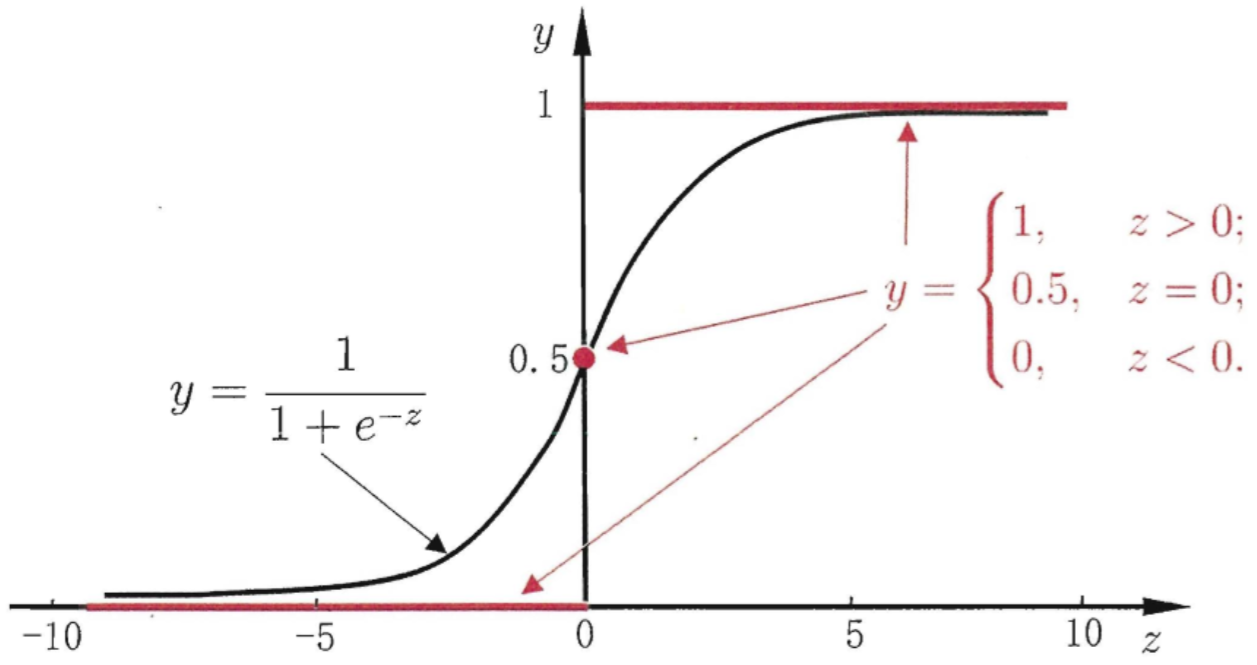
\includegraphics[width=0.7\linewidth]{Lr}
	\caption{单位阶跃函数与Logistic函数}
	\label{fig:lr}
\end{figure}
但从上图可看出,单位阶跃函数不连续,因此不能直接用作广义线性模型的联系函数. 于是我们希望找到能在一定程度上近似单位阶跃函数的"替代函数",并希望它单调可微.对数几率函数(logistic function)正是这样一个常用的替代函数:\\
\begin{equation}
y = \frac{1}{1 + e ^ {-z}}
\end{equation}
从图中可以看出,Logistic函数是一种“Sigmoid"函数,它将$z$值转化为一个接近0或1的$y$值,并且他的输出值在$z=0$附近变化很陡,由$z=w^{T}x+b$,我们得到\\
\begin{equation}y = \frac{1}{1 + e ^ {-({\bf w}^T{\bf x}+ b)}},\end{equation}
将其变化为\\
\begin{equation}
\ln \frac{y}{1-y}={\bf w}^T{\bf x}+ b
\end{equation}
将$y$视为样本${\bf x}$作为正例的可能性,则$1-y$是反例可能性,两者的比值$\frac{y}{1-y}$称为“几率”,反应了${\bf x}$作为正例的相对可能性。而对几率取对数就得到“对数几率”:
\begin{equation}
 \ln \frac{y}{1-y}
\end{equation}
由此可看出,式(5)实际上是在用线性回归模型的预测结果去逼近真实标记的对数几率,因此,其对应的模型称为"对数几率回归"(或称“逻辑回归”,logistic regression).虽然它的名字是"回归",但 实际却是一种分类学习方法.这种方法有很多优点,例如它是直接对分类可能 性进行建模,无需事先假设数据分布,这样就避免了假设分布不准确所带来的 问题;它不是仅预测出"类别",而是可得到近似概率预测,这对许多需利用概 率辅助决策的任务很有用;此外,对率函数是任意阶可导的凸函数,有很好的数 学性质,现有的许多数值优化算法都可直接用于求取最优解.
\par
将$y$视为类后验概率估计$p(y=1|{\bf x})$,则式(5)可以重写为:
\begin{equation}\ln \frac{p(y=1|{\bf x})}{p(y=0|{\bf x})}={\bf w}^T{\bf x}+ b\end{equation}
显然有
\begin{equation}p(y=1|{\bf x}=\frac{e ^ {-({\bf w}^T{\bf x}+{\bf b})}}{1 + e ^ {-({\bf w}^T{\bf x}+b)}}\end{equation}
\begin{equation}p(y=0|{\bf x}=\frac{1}{1 + e ^ {-({\bf w}^T{\bf x}+b)}}\end{equation}
于是我们可以通过极大似然法来估计${\bf w}$和$b$,给定数据集$\{(\bf { {x_i},y_i)}\}$$(i=1,2,...,m)$,Logistic regression模型最大化“对数似然”:
\begin{equation}l({\bf w},b) = \sum_{i=1}^m \ln p(y_i|{\bf x}_i;{\bf w},b),\end{equation}
即令每个样本属于其真实标记的概率越大越好.为便于讨论,令${\bm \beta} = ({\bf w},b),\hat {\bf x}=({\bf x};1)$,则${\bf w}^T{\bf x}+ b$可简写为${\bm \beta}^T \hat{\bf x}$,再令$p_1({\hat{\bf x}},{\bm \beta})=p(y=1|{\hat{\bf x}},{\bm \beta}),p_0({\hat{\bf x}},{\bm \beta})=p(y=0|{\hat{\bf x}},{\bm \beta})=1-p_1({\hat{\bf x}},{\bm \beta})$,则式(10)中的似然项可重写为
\begin{equation} 
p(y_i|{\bf x}_i;{\bf w},b)=y_ip_1({\hat{\bf x}}_i;{\bm \beta})+(1-y_i)p_0({\hat{\bf x}}_i;{\bm \beta}),
\end{equation}
将式(11)代入(10),并根据式(4)和(5)可知,最大化((10)等价于最小化
\begin{equation}l({\bm \beta})=\sum_{i=1}^m (-y_i{\bm \beta}^T{\hat{\bf x}}_i+\ln(1+e^{{\bm \beta}^T{\hat{\bf x}}_i})) \end{equation}
加入正则项$\frac{1}{C}||{\bm \beta}||_2$,上式变为:
\begin{equation}l({\bm \beta})=\sum_{i=1}^m (-y_i{\bm \beta}^T{\hat{\bf x}}_i+\ln(1+e^{{\bm \beta}^T{\hat{\bf x}}_i}))+\frac{1}{C}||{\bm \beta}||_2\end{equation}
式(13)是关于${\bm \beta}$的高阶可导连续凸函数,根据凸优化理论,经典的数值优化算法梯度下降法、牛顿法、拟牛顿法等都可求得其最优解,于是得到
\begin{equation}\bm{{\beta}^*}=\mathop{\arg\min}_{\bm \beta} l({\bm \beta})\end{equation}

\subsubsection{优缺点}
\textbf{优点:}
1)适合需要得到一个分类概率的场景。2)计算代价不高,容易理解实现。LR在时间和内存需求上相当高效。它可以应用于分布式数据,并且还有在线算法实现,用较少的资源处理大型数据。3)LR对于数据中小噪声的鲁棒性很好,并且不会受到轻微的多重共线性的特别影响。


\textbf{缺点:}
1)容易欠拟合,分类精度不高。2)数据特征有缺失或者特征空间很大时表现效果并不好。

\subsection{朴素贝叶斯}
\subsubsection{方法介绍}
朴素贝叶斯是一系列以假设特征之间强(朴素)独立下运用贝叶斯定理为基础的简单概率分类器。Sahami 最早提出了把贝叶斯 分类算法应用在垃圾邮件过滤\cite{sahami1998bayesian},并且自此朴素贝叶斯一直是垃圾邮件分类的一种基准方法。
贝叶斯分类器的思想基础:对于给出的待分类项,求解在此项出现的条件下各个类别出现的概率,哪个最大,就认为此待分类项属于哪个类别。

朴素贝叶斯分类算法\cite{langley1992analysis} 采用了变量独立假设的最初形式, 也是限制最多的一种形式, 它假设每个特征变量 $X_i$ 在 给定 类别变量 $C$ 下都是独立的。

朴素贝叶斯分类正式定义\cite{张铭锋2005垃圾邮件过滤的贝叶斯方法综述}如下:
\begin{enumerate}
	\item 设$x = \left\{ a _ { 1 } , a _ { 2 } , \dots , a _ { m } \right\}$为一个待分类项,而每个$a$为$x$的一个特征属性
	\item 类别集合,本任务只有两个类别$C = \left\{ y _ { 1 } , y _ { 2 } \right\}$
	\item 计算$P \left( y _ { 1 } | x \right) , P \left( y _ { 2 } | x \right)$
	\item 如果$P \left( y _ { k } | x \right) = \max \left\{ P \left( y _ { 1 } | x \right) , P \left( y _ { 2 } | x \right)\right\}$
\end{enumerate}
关键就是如何计算第3步中的各个条件概率,给定已知分类的待分类集合,即训练样本集;统计得到在各类别下各个特征属性的条件概率估;如果各个特征属性是条件独立的,则有如下推导:
\begin{equation}
	P \left( y _ { i } | x \right) = \frac { P ( x | y _ { i } ) P \left( y _ { i } \right) } { P ( x ) }
\end{equation}
分母对于所有类别为常数,因为我们只要将分子最大化皆可。

朴素贝叶斯的优势在于只需要根据少量的训练数据估计出必要的参数(变量的均值和方差)。由于变量独立假设,只需要估计各个变量的方法,而不需要确定整个协方差矩阵。


在scikit-learn\cite{pedregosa2011scikit}中开放了3个朴素贝叶斯的分类算法类,分别是GaussianNB,MultinomialNB和BernoulliNB。其中GaussianNB就是先验为高斯分布的朴素贝叶斯,在样本特征分布连续时表现较好,MultinomialNB就是先验为多项式分布的朴素贝叶斯,样本特征的分大部分是多元离散值,而BernoulliNB就是先验为伯努利分布的朴素贝叶斯,常用于二元离散值或者很稀疏的多元离散值。本项目使用词袋作为特征,去除了停用词和出现次数小于3的词,是离散特征,因而采用先验为多项式分布的MultinomialNB。

\subsubsection{优缺点}
\textbf{优点:}
朴素贝叶斯分类器稳定性很高效率很高,对缺失数据不太敏感,算法易于实现。算法效率很高,复杂度低,同时存储资源低,模型易于训练,超参数很少。

\textbf{缺点:}
朴素贝叶斯独立性假设过强,本任务提取的特征为词袋,很难保证词袋各个特征完全独立。需要知道先验概率,且先验概率很多时候取决于假设,本任务假设服从多项式分布。

\subsection{支持向量机}
\subsubsection{方法介绍}
支持向量机(support vector machine,SVM)是一种基于统计学习理论的模式识别方法,目前被广泛用于模式识别、文本分类以及生物信息学等多个方面。最初是被用于二分类问题,现在被广泛用于高维非线性的分类问题。它通过构造最优超平面来进行分类,它是一种特征空间上的间隔最大的线性分类器,其学习策略是间隔最大化,最终可转化为凸二次规划问题的求解。

对于线性可分得情况,它的目标是求得参数使间隔距离最大,以得到最优超平面的方程,并据此对样本进行预测分类。对于非线性可分的情况,SVM的处理方法是选择一个核函数,它的原理是用内积函数定义的非线性变换,首先将低维空间中的点映射到高维空间中,使它们在这个高维空间中线性可分,然后再使用线性划分的原理判断分类边界,在这个空间中求(广义)最优分类面。此外,核函数能够使得高维空间中的所有运算都可以在低维空间中进行,从而省去了计算映射的过程,也避免了增加运算复杂度。

垃圾邮件过滤任务是线性不可分的情况,使用的SVM为线性支持向量机。

线性支持向量机是在线性可分支持向量机基础上推广,它是针对的是线性不可分的问题。所谓的线性不可分指的是空间上有两类,在空间找不到任何的分割平面能把这两类绝对完全分开,总会有一些落到决策边界内或被分错。这时按照线性可分支持向量求解就找不到合适的超平面来将两类有效的区分开来,针对这类问题可以使用线性支持向量机——在合理的误分类条件下,找到边缘距离较大且误分点到边缘距离较小的超平面,对原本线性可分支持向量机的约束做松弛,以适应放非线性可分数据,这时我们引入松弛变量$\xi$来实现,如下式所示:
\begin{equation}\label{equ:PixelColorContrast}
   y_{i}(w \cdot x_{i} + b) \geq 1-\xi_{i}
\end{equation}
这里的$\xi_{i}$就是松弛变量,也就是说对于每一个分错的点,都要付出一个代价,此外,对于任意$\xi_{i}$都有$\xi_{i} \geq 0$。

\subsubsection{优缺点}
\textbf{优点:}
SVM使用核函数可以向高维空间进行映射,进而可以解决非线性的分类,当核函数已知时,可以简化高维空间问题的求解难度。它的分类思想很简单,就是将样本与决策面的间隔最大化,但却具有较好的分类效果。

\textbf{缺点:}
SVM对大规模数据训练比较困难。且无法直接解决多分类问题,只能用用间接的方法来做,但本任务是二分类的,所以不存在这一问题。

\subsection{卷积神经网络}
\subsubsection{方法介绍}
卷积神经网络(CNN)被广泛应用于计算机视觉领域,Kim等人\cite{kim2014convolutional}将CNN应用于文本分类,并在该领域取得了state-of-the-art的效果,从此CNN在自然语言处理领域获得了广泛的关注。本次实验中,我们选用了zhang等人\cite{zhang2015sensitivity}所提出的模型架构用于垃圾短信识别。

在经过文本预处理步骤后,垃圾短信被表示为一连串的词语。首先,我们将其转换为句子矩阵,其中每一行是每个词语的向量化表达,我们采用预训练的word embedding来初始化这一向量表示。假设$d$为词向量的维度,且句子长度为$s$,则句子矩阵的维度为$s \times d$。在这个句子矩阵上,我们利用卷积神经网络来提取与垃圾短信相关联的特征用于分类。假设卷积核的权值矩阵为$\mathbf{w}$,其宽度为$h$。由于自然语言的序列性质,我们采用1D卷积核,则$\mathbf{w} \in \mathcal{R}^{h \times d}$。令句子矩阵$\mathbf{A} \in \mathcal{R}^{s \times d}$,并且用$\mathbf{A}[i:j]$来代表$\mathbf{A}$来代表$\mathbf{A}$从$i$行到$j$行的子矩阵。卷积操作的输出序列$o \in \mathcal{R}^{s-h+1}$由公式\eqref{cnn1}计算获得:
\begin{equation}\label{cnn1}
    o_i = \mathbf{w} \cdot \mathbf{A}[i:i+h-1]
\end{equation}
其中$i = 1 ... s-h+1$,我们对每一个$o_i$添加偏置项$b\in\mathcal{R}$以及激活函数$f$,则该卷积核产生的特征向量$c\in \mathcal{R}^{s-h+1}$为:
\begin{equation}\label{cnn2}
    c_i = f(o_i + b)
\end{equation}
在实验中,为了提取更丰富的特征,我们采用了许多不同长度的卷积核。

提取的特征向量的维度依赖于$h$和$s$,由于不同句子的长度不用,最终产生的特征向量的维度是不确定的,这将对进一步的分类器的构建造成困难;另一方面,众多卷积核提取的特征向量维度过高,不利于分类器选取显著特征。为了解决这些问题,我们对每个卷积核提取的特征向量进行1-max池化\cite{boureau2010theoretical},通过这种操作,我们可以选取出每个卷积核提取出的最显著的特征,再这之后,我们将池化后选出来的显著特征进行拼接,得到了长度为$n$的特征$z$,其中$n$为卷积核的个数。并将这一特征送入一个全连接的输出层,进行二分类,如公式\eqref{cnn3}所示:
\begin{align}\label{cnn3}
    \hat{y} = \sigma(W^oz + b)
\end{align}
其中$\hat{y}$为标签的估计值,$W^o$和$b$为输出层的参数,$\sigma$为sigmoid函数,$z$为1-max池化输出的特征向量。

模型使用交叉熵损失函数,并利用Adam\cite{kingma2014adam}进行优化。为了防止过拟合,模型在输出层之前以及词嵌入层之后使用了Dropout\cite{hinton2012improving},这种技术按照预设的概率随机地将矩阵的一些值设为零,除此之外我们还使用了L2正则化。

\subsubsection{优缺点}
\textbf{优点:}
卷积神经网络的优势在于对于n-gram特征强大的提取能力,通过堆叠多层卷积层,模型可以学习到文本高层次的特征,除此之外,卷积网络可以通过并行计算来提高计算速度。

\textbf{缺点:}
相比于循环神经网络,卷积神经网络更难学习到文本中的长期依赖性。

\subsection{循环神经网络}
\subsubsection{方法介绍}
循环神经网络(RNN)主要解决序列数据的处理,比如文本、语音、视频等等。这类数据的样本间存在顺序关系,每个样本和它之前的样本存在关联。比如说,在文本中,一个词和它前面的词是有关联的;在气象数据中,一天的气温和前几天的气温是有关联的。不同于传统的前向反馈神经网络(Feed-forward Neural Networks,FNNs),RNN引入了定向循环,能够处理那些输入之间前后关联的问题。因此能够很好地学习到其中包含的信息依赖关系,当前,RNN已经在自然语言处理(Natural Language Processing, NLP)等领域中取得了巨大成功以及广泛应用。

在经过简单的文本预处理后,对其中的标点和繁体字符进行了相应的转换。在实验中发现,相比于使用Jieba对短信内容进行分词,直接使用一层RNN网络来学习词语级别信息能够更好地对短信内容特征进行抽取。因此,我们直接对文本进行字符级别的处理,首先对训练集中短信文本进行单字拆分并对其中字符进行统计,获取其中频度最高的前$k$个构建词汇表$V$。接着使用随机初始化训练得到的word embedding对表示词汇表中词汇$e$,设其词向量维度为$d$。在对短信文本进行填充对齐后,固定其长度为$l$,由此将短信内容表示为$l\times $的矩阵$M$。接着,我们将句子矩阵$M$输入至两层RNN网络中,对应字到词、词到句的特征抽取。网络中使用LSTM核,若前一时刻状态为$C_{t-1}$,$f_t$为遗忘$t-1$时刻内容的概率,则可由公式\eqref{rnn1}得到当前状态$C_t$
\begin{align}\label{rnn1}
    C_t = C_{t-1} * f_t + i_t*\hat{C_t}
\end{align}

其中$i_t$和$\hat{C_t}$分别为使用Sigmod和tanh作为激活函数得到的当前时刻信息。

同时,当前时刻的输出$h_t$可由$t-1$时刻输出$h_{t-1}$和当前时刻输入$e_t$得到,其计算方法如公式\eqref{rnn2}:
\begin{align}\label{rnn2}
    h_t = Sigmod(W[h_{t-1}, e_t]+b) * tanh(C_t)
\end{align}

之后,我们将RNN网络得到的短信信息表达输入到ReLU激活函数中,并通过Softmax函数实现对短信文本的二分类。

模型也使用交叉熵作为损失函数,并且在每层RNN网络和RelU激活函数之后都使用Dropout来防止模型过拟合。

\subsubsection{优缺点}
\textbf{优点:} 循环神经网络最大的优点在于能够学习到句子中存在的长期依赖性,而LSTM模型中遗忘门结构能够去除其中的无效信息,由此能够对一些较长且隐蔽的短信文本进行正确分类。

\textbf{缺点:} RNN训练时无法并行操作,导致训练速度相比于CNN更慢,同时其对带宽内存等资源消耗较大,系统调参方面有着较大的限制。



\subsection{模型线性融合}
\subsubsection{方法介绍}
首先我们通过一个例子证明集成能取得好的效果,如下图所示,平面上分布着一些待分类的点。如果要求只能用一条水平的线或者垂直的线进行分类,那不论怎么选取直线,都达不到最佳的分类效果。但是,如果可以使用集体智慧,比如一条水平线和两条垂直线组合而成的图中折线形式,就可以将所有的点完全分开,得到了最优化的预测模型。
\begin{figure}[H]
	\centering
	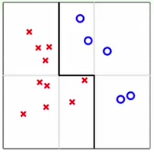
\includegraphics[scale=0.3,width=0.3\linewidth]{ensemble}
	\caption{集成示意图}
	\label{fig:ensemble}
\end{figure}
这个例子表明,通过将不同的假设以一定方式结合起来,得到了比单一假设更好的预测模型。这就是集成的优势所在,它拓展了模型的复杂度,提高了预测模型的能力,起到了特征转换的效果。

本文采取的线性融合的方法,对于每一个分类器$g_t$,给出它的权重$\alpha_t$,线性融合模型如下所示:
\begin{equation}
G(x) = sign\bigg(\sum_{t=1}^{T}\alpha_t  g_t(x)\bigg)\ ,\ \alpha_t \ge 0
\end{equation}
对于$\alpha_t$的选择,本文采用Logistic regression模型,将不同模型在训练集上的预测结果作为LR集成模型的输入,拟合训练集的真实的Lable,学习得到不同模型的参数,然后在验证集做实验,得到验证集上的评价指标;对于所需要集成的模型,本文选择在验证集上表现最好的三个模型CNN、LSTM、Random Forests作为分类器。本文在实验过程中发现加入其他模型如SVM、Naive Bayes等在验证集上表现较差的模型,LR集成模型学得的其他模型的权重为负值或者与这三者相比权重较小,加入表现差的模型后,整体的集成结果也变差。采用表现最好的CNN、LSTM、Random Forests作为分类器,通过学习三者的权重,集成模型在验证集上的表现(垃圾短信作正例时的F1-score与非垃圾短信作正例时的F1-score)优于所有单个分类器模型。
\subsubsection{优缺点}
\textbf{优点:}
1)集成 models 有助于防止欠拟合(underfitting)。它把所有比较弱的分类器g(t) 结合起来,利用集体智慧来获得比较好的模型 G 。集成就相当于是特征转换,来获得复杂的学习模型。
2)集成 models 有助于防止过拟合(overfitting)。它把所有分类器 g(t) 进行组合,容易得到一个比较中庸的模型,类似于SVM的最大间隔一样的效果,从而避免一些极端情况包括过拟合的发生。从这个角度来说,集成起到了正则化的效果。
由于集成具有这两个方面的优点,所以在实际应用中集成 models 都有很好的表现。

\textbf{缺点:}
1)增加了一次训练过程;2)需要所有其他单模型的分类结果。



\section{实验} 

\subsection{实验设置}

\subsubsection{数据集划分}
本次实验中,我们采用五折交叉验证来划分数据集,其中80\%的数据作为训练集,10\%的数据作为验证集进行超参数调整,剩余10\%的数据作为测试集。所有结果均为五折测试集结果的平均值。

\subsubsection{评价指标}
由于垃圾短信数据集中,垃圾短信类别和非垃圾短信类别的样本数目不平衡,我们采用了精确率(Precision),召回率(Recall)和F1来评估各种方法的分类效果。
\begin{align}
    \begin{split}
        Precision = \frac{TP}{TP + FP} \\
        Recall = \frac{TP}{TP + FN} \\
        F1 = 2\cdot\frac{Precision \times Recall}{Precision + Recall}
    \end{split}
\end{align}
其中给定类别,TP是预测为该类别且真实为该类别的样本数目,FP是预测为该类别且真实不是该类别的样本数目,FN为预测为不是该类别且真实为该类别的样本数目。

\subsubsection{参数设置}


\textbf{随机森林(RF)} 我们首先从句子中抽取3000维的TF-IDF特征,并将其输入到随机森林模型中进行训练。其中,随机森林模型采用随机且有放回地抽样,树的数量为100,使用基尼系数作为特征选择的评价标准,并使用Out-of-Bag(OOB)来估计泛化误差。

\textbf{逻辑斯蒂回归(LR)} 采用拟牛顿方法中的lbfgs方法,正则项系数C设置为1。

\textbf{朴素贝叶斯(NB)} 
实现时使用的是sklearn的naive\_bayes库的MultinomialNB,并设置平滑项参数$\alpha$为1。

\textbf{支持向量机(SVM)} 
考虑到训练速度的问题,在具体实现时使用的是sklearn的liblinear库中的LinearSVC:对错误分类的惩罚的松弛变量为0.6,停止训练的误差值大小1e-4,损失函数选择hinge loss。

\textbf{卷积神经网络(CNN)} 经过超参数搜索后,我们在数据集上训练了word2vec,并将之用于embedding layer的初始值。除此之外,我们还随机初始化了300维的word embedding,并将其与预训练的word embedding进行连接。word2vec我们使用了gensim\footnote{https://radimrehurek.com/gensim/index.html}的实现,并设置为gensim库的默认参数。我们设置dropout为0.1,L2正则化比例为1e-5,卷积核个数为150,使用大小为2,3,4,5的卷积核,学习率设置为2e-5,并过滤出现次数小于3的词语。



\textbf{循环神经网络(RNN)}
由于从字符层面对短信文本进行分词,得到词汇表大小仅为5000,所以我们将词向量维度设置为64,以提高训练速度,同时减小资源消耗。另外,在进行参数调整优化后,我们将句子长度设置为300,学习率设置0.001,dropout比例设置为0.1,隐藏层神经元个数设置为128。

\textbf{集成模型(Ensemble)} 训练CNN、LSTM、RF模型的权重时用logistic regression方法,采用拟牛顿方法中的lbfgs方法,正则项系数C设置为0.05。

\subsection{实验结果}
\begin{table}[!t]
	\renewcommand{\arraystretch}{1.2}
    \caption{各方法对垃圾短信识别效果的比较}
    \label{table:result}
    \centering
    \begin{tabular}{{|c|c|c|c|c|c|c|}}
        \hline
        \multirow{2}{*}{模型}
          & \multicolumn{3}{c|}{垃圾短信} & \multicolumn{3}{c|}{非垃圾短信} \\
          \cline{2-7}
          & Precision & Recall & F1 & Precision & Recall & F1 \\ \hline \hline
    CNN & \textbf{0.9976} & 0.9895 & 0.9935 & 0.9988 & \textbf{0.9997} & \textbf{0.9993} \\ \hline
    RNN & 0.9954 & 0.9668 & 0.9809 & 0.9963 & 0.9995 & 0.9979 \\ \hline
    NB & 0.8665 & 0.9807 & 0.9201 & 0.9978 & 0.9831 & 0.9904 \\ \hline
    RF & 0.9957 & 0.9828 & 0.9892 & 0.9981 & 0.9995 & 0.9988 \\ \hline
    LR & 0.9739 & 0.9608 & 0.9673 & 0.9956 & 0.9971 & 0.9964 \\ \hline
    SVM & 0.9959 & 0.9839 & 0.9899 & 0.9982 & 0.9995 & 0.9989  \\ \hline
Ensemble & 0.9971 & \textbf{0.9905} & \textbf{0.9938} & \textbf{0.9989}  & \textbf{0.9997} &  \textbf{0.9993}\\ \hline
    \end{tabular}
\end{table}
各方法在垃圾短信识别数据集上的结果如表\ref{table:result}所示,由表\ref{table:result}的结果可以看到:一方面,绝大多数模型在该任务上都达到了近乎完美的分类效果,即使是简单的逻辑斯蒂回归模型,在垃圾短信类别和非垃圾短信类别的F1值也分别超过了0.967和0.996,这说明垃圾短信分类任务是一种较为简单的文本分类任务;另一方面,垃圾短信类别的分类效果均落后于非垃圾短信类别,这主要是由于数据集的不平衡引起的。尽管试验中采用了一定程度的措施来缓解数据不平衡问题,但依然无法完全避免这一现象的发生。

在单模型中,CNN取得了最好的效果,这证明了深度学习方法在垃圾短信分类任务的强大能力,也应证了\cite{kim2014convolutional, zhang2015sensitivity}等的研究结果。深度学习方法中,CNN的分类效果超越了基于字符的RNN,这可能表明在垃圾短信识别领域,相比于捕获语言的长期依赖性,模型提取n-gram特征的能力更为重要,也从侧面表明垃圾短信识别任务并不需要对文本的深层次理解。经典模型当中,SVM和RF的效果几乎相当,SVM略胜一筹。

尽管只采用了简单的线性集成方法,集成模型的效果依然超过了所有的单模型。这一结果是令人鼓舞的,这表明在该数据集上,模型的效果依然有改进的潜力。

\subsection{Demo展示}
Demo系统采用前后端分离的方式编写。前端负责接收用户的输入并传送给后端,后端经过解析处理将结果返回给前端,最后前端将结果展示给用户。前后端之间通过JSON进行数据交换,这种解耦合的方式让整个系统具有极大的灵活性。

\subsubsection{前端}
前端采用Vue\footnote{https://vuejs.org}框架编写。Vue是基于JavaScript编写的一套渐进式框架。Vue由数据驱动, 当数据改变,界面也随之改变。相对于其他框架,Vue更加简洁易写,能较快地搭建出原型, 进行实验分析。

\subsubsection{后端}
后端采用Flask\footnote{http://flask.pocoo.org}框架编写。Flask是一个使用Python编写的轻量级Web应用框架。其WSGI 工具箱采用Werkzeug,模板引擎则使用Jinja2。Flask使用BSD授权。Flask也被称为 “microframework”,因为它使用简单的核心,用extension增加其他功能。Flask没有默认使用的数据库、窗体验证工具。

\subsubsection{使用说明}
Demo系统如图\ref{fig:demo}所示,系统的网址为 \url{http://spam.zengyutao.me:5000}。由于系统部署在实验室服务器中,所以系统暂时只能在计算所网数实验室内网内访问。同时因为深度学习模型占显存比较大,暂时是关闭的\footnote{如果需要检查可以联系陶舒畅同学把它打开}整个系统由三部分组成。

\textbf{第一部分}
Demo系统介绍区域。该系统的名字叫“WHAT ARE WE CALLING”,同时这也是我们小组的名字。

\textbf{第二部分}
用户输入区域,主要元素为输入文本框及按钮。用户可在该区域输入要识别的文本,并按回车键或者点击文本框后的按钮,就能将信息发送给后端处理。

\textbf{第三部分}
结果展示区域。该区域主要由两部分组成,分别是用户输入展示和文本识别展示。用户输入展示部分显示用户即时的输入,即用户所要识别的文本。文本识别展示部分显示每一个模型对用户输入所判定的结果,该结果用表格来表示。其中,主要包含三个元素,分别是模型的名字,判定为垃圾短信的概率,判定为非垃圾短信的概率。

\begin{figure}[ht]
	\centering
	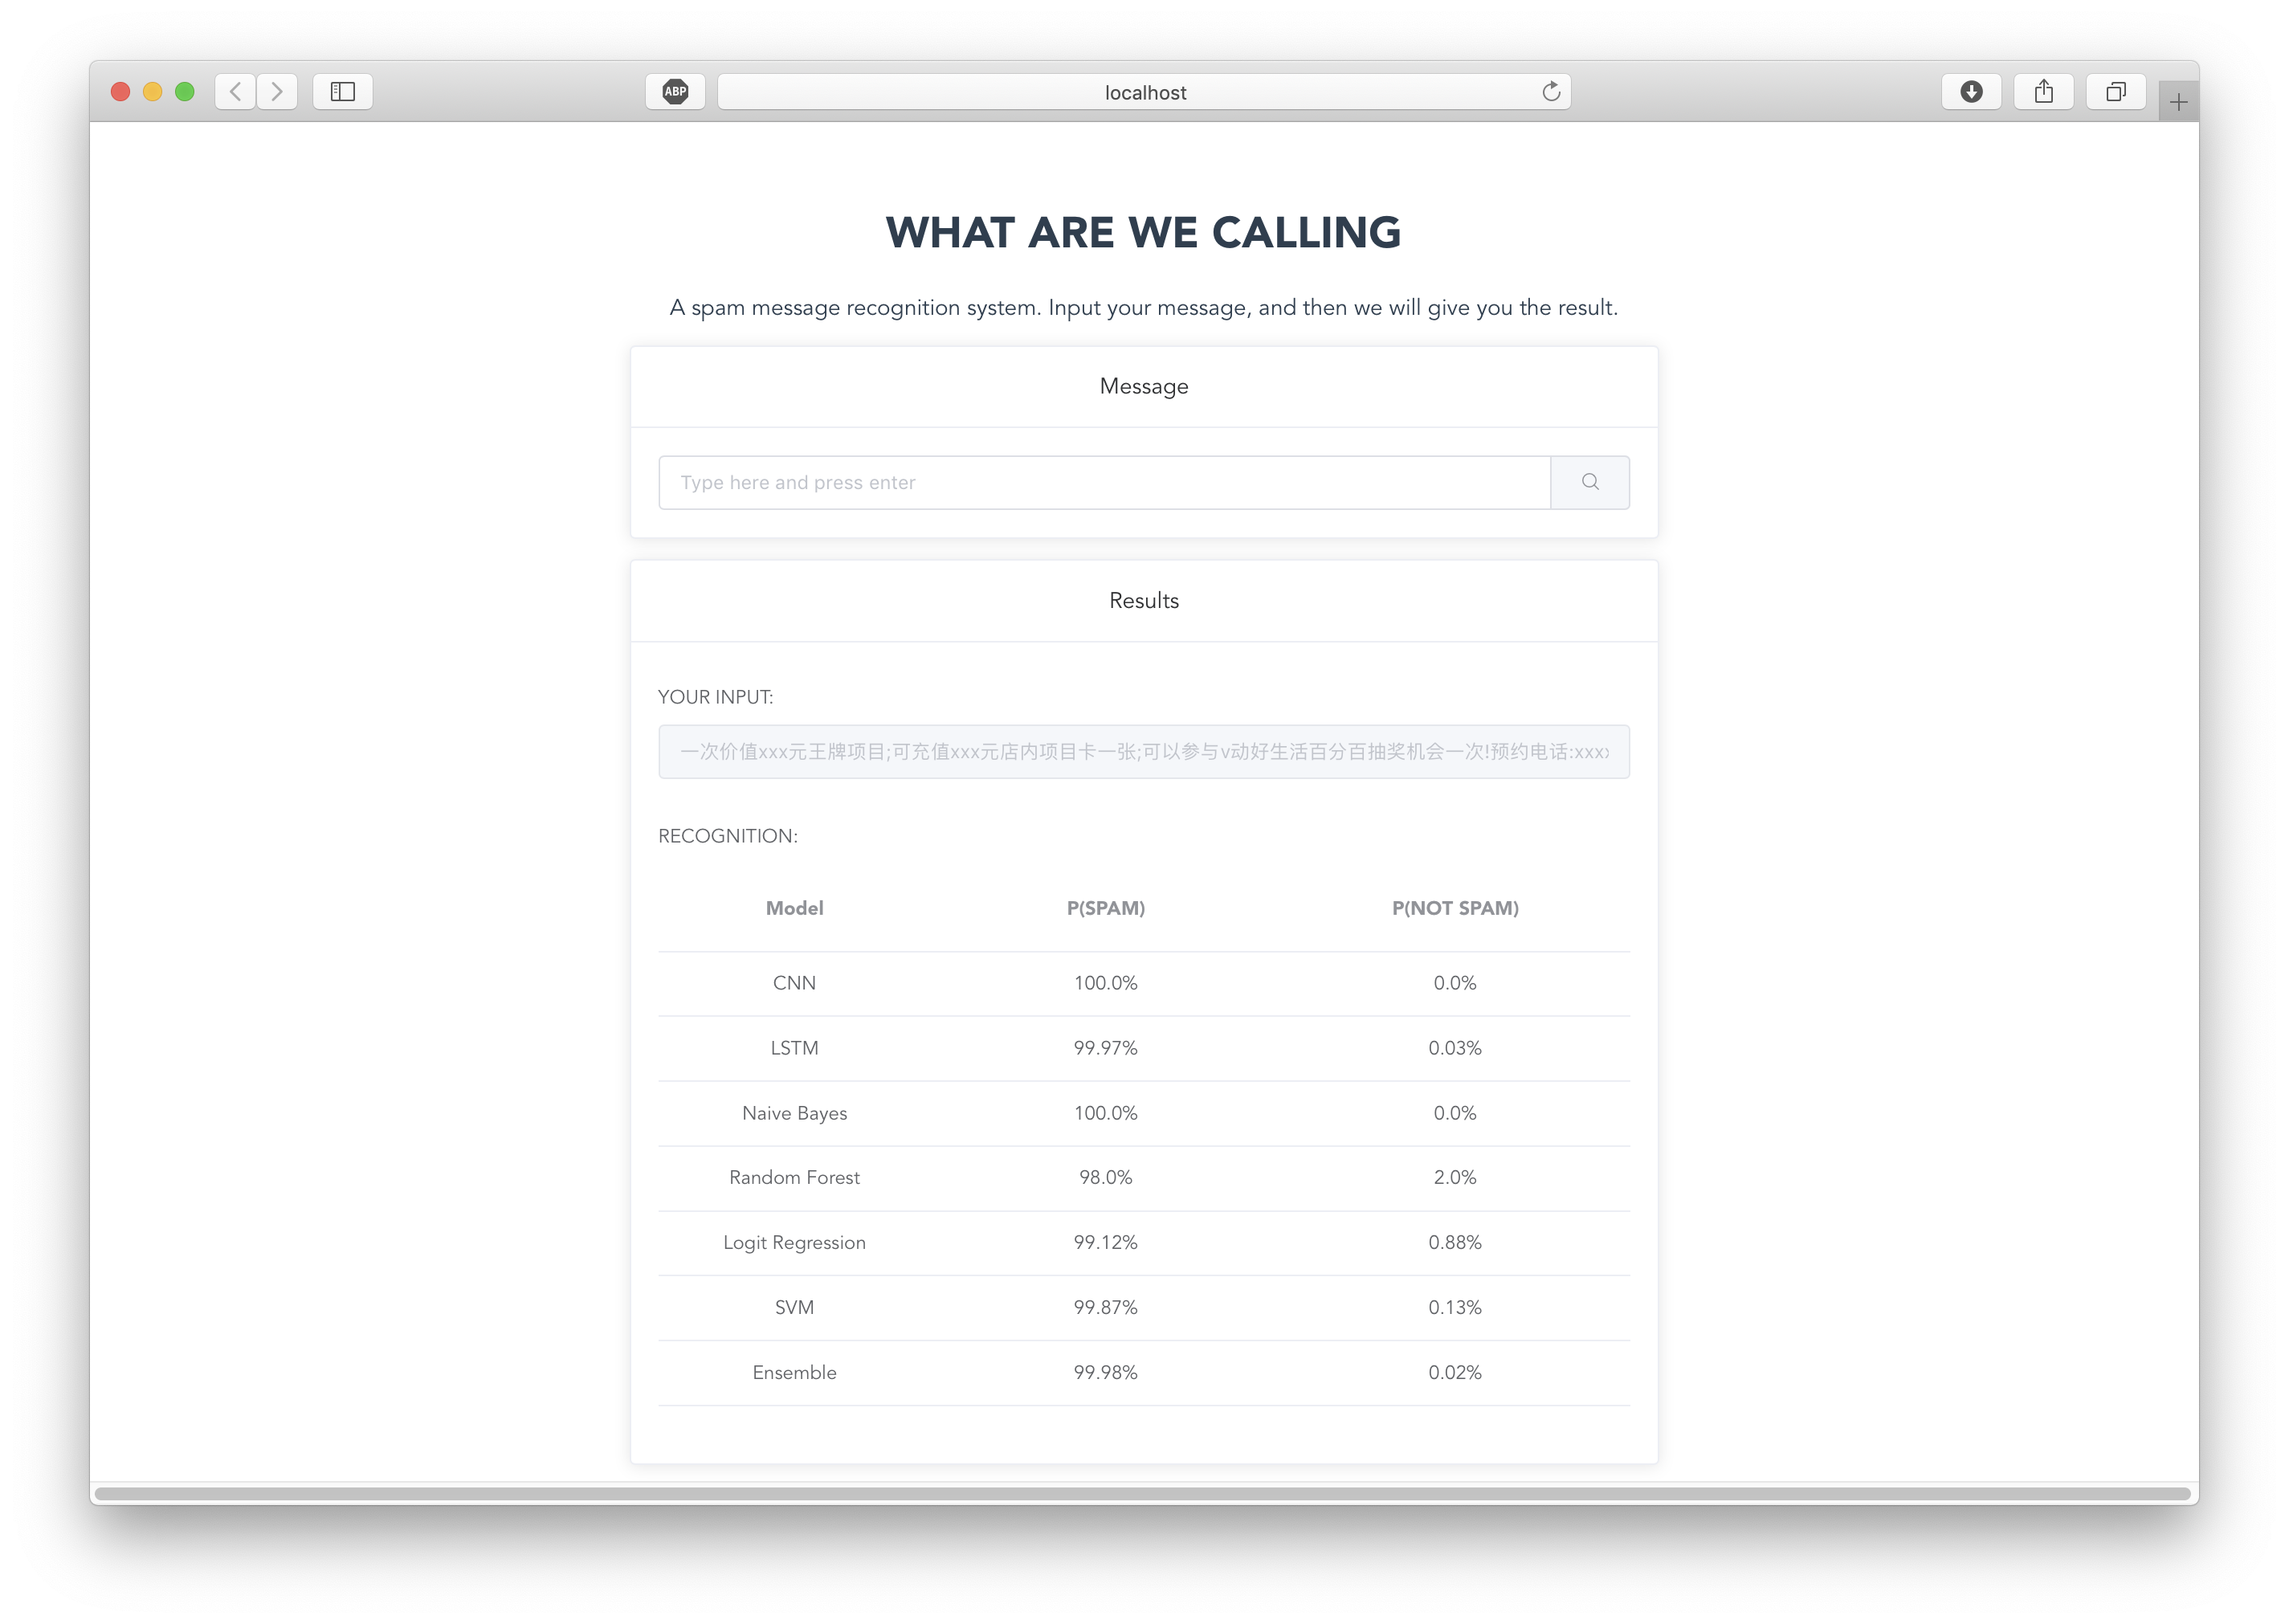
\includegraphics[scale=0.4,width=1.0\linewidth]{demo.png}
	\caption{Demo系统界面}
	\label{fig:demo}
\end{figure}
\section{总结及讨论}
\subsection{项目总结}
近年来,垃圾短信不断泛滥,给人们生活带来了很大困扰,高效的识别垃圾短信已经成为日常生活的重要技术,垃圾短信的识别可以对短信文本分类来实现。我们对比了文本分类问题和图像分类以及推荐系统的异同点,并根据文本分类的特点选取了6个模型进行实现。

垃圾短信识别是一个经典的文本分类任务,传统的机器学习方法在分类器方面和特征提取方面在该任务上已经有了较好的效果,深度学习方法应用于该任务,更取得了不小进展。

本项目首先进行了文本的预处理使用正则化,分词,词向量化等方式,将原始语料处理成便于应用机器学习算法的相对规则化的数据。然后提取了TF-IDF特征,哈希特征用于经典的机器学习算法。

本项目共实现了六个模型,其中包括经典的机器学习方法逻辑回归、朴素贝叶斯、支持向量机、随机森林,两个深度学习算法卷积神经网络和循环神经网络,并将模型进行集成,对比了各自的优缺点,并使用所给数据集进行了实验以及参数的调整。在单模型中,CNN取得了最好的效果,这证明了深度学习方法在垃圾短信分类任务的强大能力,而集成模型的效果超过了所有的单模型。同时我们实现了Demo,部署在了计算所网数实验室服务器上。


\subsection{模型改进}
\begin{itemize}
    \item 实验中,对分类错误样本的分析后发现,存在较多分词错误导致的错误分类,在未来可以通过整理垃圾短信词表,或本地训练分词模型等方式来改进分词的精确度。
    \item 由于很多垃圾短信用词和行文并不规范,可能存在难以避免的分词错误。为尽量减轻这一影响,对于卷积神经网络,可以引入字符级别的embedding表示。
    \item 由于设备性能的限制,随机森林中树的数量只设置了100棵,TF-IDF特征只选取3000维。如果在计算资源充足的条件下,增大森林规模和特征多样性,可能会给模型带来一定的提升。
    \item 对于部分传统模型,如逻辑斯蒂回归,朴素贝叶斯等,可以通过卡方检验、互信息等方式过滤掉无用的词项特征,提高准确度和效率,对于其他传统模型而言,这种方式也可以提高它们的计算效率。
    \item 虽然在该数据集上,大多数模型都达到了近乎完美的分类效果,不需要引入更多的关于主题方面的特征,但在其他数据集上的情形未知,可以通过LDA等主题模型来学习文本的主题分布,作为附加特征辅助分类。
\end{itemize}




\clearpage
% -----------------------------------REFERENCE----------------------------------------
\bibliography{citation}
\addcontentsline{toc}{section}{参考文献}
\end{document}

